% Romer 2.12 (with 2.10-2.11 as far as needed). Checked by check-2-12-11-1.py; the figures plot its paths.
\problema{Romer 2.12}{Temporary taxes on investment income}{p.~96}{Romer \S2.6--2.7, problems 2.10--2.11}
Notation of Romer ch.~2: $k$ and $c$ per unit of effective labor, no depreciation, CRRA utility with
coefficient $\theta$, and $\rho-n-(1-\theta)g>0$. Investment income is taxed at $\tau(t)\in\{0,\tau\}$,
$0<\tau<1$, and the revenue is rebated lump-sum (the setting of 2.10). Problems 2.10--2.11 are solved
only as far as 2.12 needs them.

\passo{The two systems of dynamics (2.10a)}{A household holding $k_h$ has the flow budget
$\dot k_h=(1-\tau(t))f'(k)k_h+w+T-c-(n+g)k_h$, with wage $w=f(k)-kf'(k)$ and a transfer
$T=\tau(t)f'(k)k$ that does not depend on its own $k_h$. Its Euler equation is Romer's (2.20) with the
after-tax return $r(t)=(1-\tau(t))f'(k(t))$; imposing $k_h=k$ in the budget,
\[ \begin{aligned}
\frac{\dot c}{c}&=\frac{(1-\tau(t))f'(k)-\rho-\theta g}{\theta},\\
\dot k&=(1-\tau)f'(k)k+\bigl[f(k)-kf'(k)\bigr]+\tau f'(k)k-c-(n+g)k=f(k)-c-(n+g)k.
\end{aligned} \]
The tax drops out of the resource constraint, so the $\dot k=0$ locus $c=\bar c(k)\equiv f(k)-(n+g)k$
does not move. The $\dot c=0$ locus moves from $f'(k^*)=\rho+\theta g$ to
$f'(k_\tau)=(\rho+\theta g)/(1-\tau)>\rho+\theta g$; as $f''<0$, $k_\tau<k^*$: the vertical line shifts
left. Call N the untaxed system (steady state $E=(k^*,c^*)$, saddle path $S_N$) and T the taxed one
($E_\tau=(k_\tau,c_\tau)$, saddle path $S_T$). Since $\rho+\theta g>n+g$, $f'(k^*)>n+g=f'(k_{GR})$, so
$k^*<k_{GR}$, $\bar c$ is increasing on $(0,k^*]$ and $c_\tau<c^*$.}

\passo{Regions and traps}{Under T, $\dot c<0$ iff $k>k_\tau$, and $\dot k<0$ iff $c>\bar c(k)$. Let
\[ A=\{k>k_\tau,\ c>\bar c(k)\},\qquad B=\{k>k_\tau,\ c<\bar c(k)\},\qquad C=\{k<k_\tau,\ c>\bar c(k)\}: \]
in $A$ both variables fall; in $B$, $c$ falls and $k$ rises; in $C$, $c$ rises and $k$ falls.
$B$ and $C$ are traps. In $B$, $k$ rises, so
$k_\tau$ is never reached, and on the locus the motion is straight down, back into $B$. In $C$, $k$
falls, and $c$ rises while $\bar c(k)$ falls with $k$, so neither boundary is ever reached. $A_N$, $B_N$,
$C_N$ are the same regions under N, with $k^*$ in place of $k_\tau$. Along $S_N$, $c$ and $k$ move
together toward $E$, so $S_N$ is increasing; it lies strictly below $\bar c$ for $k<k^*$ (there
$\dot k>0$) and above $c^*$ for $k>k^*$.}

\passo{What can jump, and when (2.11b)}{$k$ is a stock with finite $\dot k$, so it is continuous. For $c$,
Romer's (2.18) gives $\theta\ln c(t)=\ln B-\ln\lambda-\beta t+R(t)-(n+g)t$, with
$R(t)=\int_0^t r(s)\,ds$. $R$ is continuous even at the dates where $r$ jumps (the start or end of the
tax), so for a given $\lambda$ the path of $c$ is continuous. The multiplier $\lambda$, the marginal
utility of initial wealth, is set when the plan is made and changes only when news arrives. Here the
only news date is $0$, so $c$ can jump at $0$ and nowhere else. In words: a foreseen upward jump at
$t'$ would let the household gain a first-order amount of utility by moving consumption from just
after $t'$ to just before it, at a negligible cost in interest.}

\passo{Where the economy must be when the last regime starts}{After the last change of regime, N
governs forever and Romer's \S2.3 argument applies: above $S_N$, $k$ hits zero in finite time and $c$
would then have to jump down (ruled out above); below $S_N$, $c\to0$ while $k$ rises past $k_{GR}$, and
households hold capital whose present value never vanishes, violating the transversality condition.
So at the date of the last change the economy must be on $S_N$. Neither $k$ nor $c$ jumps at that
foreseen date, so the dynamics of the preceding regime must carry it onto $S_N$ exactly then ($S_N$ is
not invariant under T, so arriving early does not help). With a permanent tax the target is $S_T$
instead: in 2.10(b) $c$ jumps at $0$ straight onto $S_T$; in 2.11 it jumps by less at $0$, drifts
northwest under N and reaches $S_T$ exactly at $t_1$.}

\parte{a}
\passo{Regimes}{T on $[0,t_1)$, N from $t_1$ on, news only at $0$. So $c$ jumps at $0$ to some $c_0$,
both variables are continuous at $t_1$, and the T-trajectory from $(k^*,c_0)$ must be on $S_N$
exactly at $t_1$.}
\passo{The jump is upward}{If $c_0<c^*$, the point $(k^*,c_0)$ is in $B$; if $c_0=c^*$, it is on the
locus with $\dot k=0>\dot c$ and enters $B$ at once. Either way the path is trapped in $B$, with
$k(t)>k^*$ and $c(t)<c^*$ for all $t>0$, while $S_N$ lies above $c^*$ wherever $k>k^*$: $S_N$ is never
reached. Hence $c_0>c^*$.}
\passo{Dynamics while the tax is in force}{$(k^*,c_0)$ is in $A$, so $c$ and $k$ both start to fall.
If the path stayed in $A$ until $t_1$, it would be above $\bar c$ at some $k<k^*$, where $S_N$ lies
below $\bar c$; if it entered the trap $C$, it would stay above $\bar c$ for good. So it must cross the
$\dot k=0$ locus into $B$ at some $t_m<t_1$, at $k_m\in(k_\tau,k^*)$; from then on $c$ keeps falling
while $k$ rises. At $t_1$, $c(t_1)<c(t_m)=\bar c(k_m)<\bar c(k^*)=c^*$, and since $S_N$ is increasing,
$k(t_1)<k^*$. A path starting on or above $S_T$ cannot cross $S_T$ and never enters $B$, so $c_0$ lies
strictly between $c^*$ and the height of $S_T$ at $k^*$: the jump is smaller than under the permanent
tax of 2.10(b). By continuity some $c_0$ in that interval arrives on $S_N$ exactly at $t_1$ (the
arrival time tends to $0$ as $c_0\downarrow c^*$ and to infinity as $c_0$ approaches $S_T$).}
\passo{After the tax is removed}{The economy rides $S_N$ up to $E$: $c$ and $k$ both rise. At $t_1$ the
$\dot c=0$ line jumps back from $k_\tau$ to $k^*$, so $\dot c$ switches from negative to positive (a
kinked trough in $c$), while $\dot k=f(k)-c-(n+g)k$ is continuous ($k$ is smooth). In sum: $c$ jumps up
at $0$, falls throughout the tax period to below $c^*$ and then rises back to $c^*$; $k$ falls to a
minimum at $t_m<t_1$, is already rising when the tax ends, and returns to $k^*$.}

\begin{center}
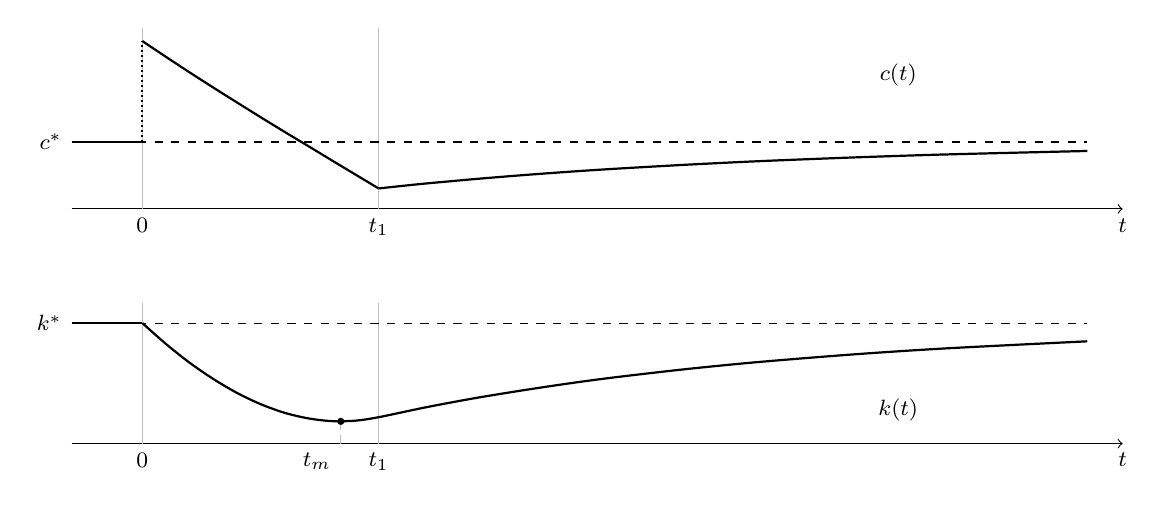
\begin{tikzpicture}[x=0.3cm,font=\footnotesize]
\begin{scope}[y=0.17cm]
  \draw[->] (-3,-5) -- (41.5,-5) node[below]{$t$};
  \foreach \x/\l in {0/0,10/t_1} \draw[gray!50] (\x,-5) node[below,black]{$\l$} -- (\x,8.5);
  \draw[dashed] (-3,0) node[left]{$c^*$} -- (40,0);
  \draw[thick] (-3,0) -- (0,0);
  \draw[thick,densely dotted] (0,0) -- (0,7.54);
  \draw[thick] plot[smooth] coordinates {(0,7.54) (1,6.36) (2,5.20) (3,4.07) (4,2.96) (5,1.86) (6,0.78) (7,-0.28) (8,-1.35) (9,-2.41) (10,-3.47)};
  \draw[thick] plot[smooth] coordinates {(10,-3.47) (11,-3.28) (12,-3.10) (14,-2.78) (16,-2.49) (18,-2.23) (20,-2.00) (23,-1.70) (26,-1.44) (30,-1.16) (34,-0.93) (40,-0.67)};
  \node at (32,5) {$c(t)$};
\end{scope}
\begin{scope}[yshift=-2.3cm,y=0.17cm]
  \draw[->] (-3,-9) -- (41.5,-9) node[below]{$t$};
  \foreach \x/\l in {0/0,10/t_1} \draw[gray!50] (\x,-9) node[below,black]{$\l$} -- (\x,1.5);
  \draw[gray!50,densely dashed] (8.4,-9) node[below left,black]{$t_m$} -- (8.4,-7.34);
  \draw[dashed] (-3,0) node[left]{$k^*$} -- (40,0);
  \draw[thick] (-3,0) -- (0,0);
  \draw[thick] plot[smooth] coordinates {(0,0.00) (1,-1.56) (2,-2.96) (3,-4.17) (4,-5.21) (5,-6.05) (6,-6.69) (7,-7.11) (8,-7.32) (9,-7.29) (10,-7.03) (12,-6.29) (14,-5.63) (16,-5.05) (18,-4.52) (20,-4.05) (23,-3.44) (26,-2.92) (30,-2.35) (34,-1.89) (40,-1.36)};
  \fill (8.4,-7.34) circle (1.3pt);
  \node at (32,-6.5) {$k(t)$};
\end{scope}
\end{tikzpicture}\par
{\footnotesize (a): tax on $[0,10)$. Simulated paths ($f=k^{1/3}$, $\rho=0.04$, $\theta=2$, $n=0.01$,
$g=0.02$, $\tau=0.3$), plotted as $100\ln(c/c^*)$ and $100\ln(k/k^*)$; dotted: the jump at $0$.}
\end{center}

\intuicao{While the tax is in force the after-tax return is below $\rho+\theta g$, so the Euler equation
makes consumption fall; once it is lifted, capital is scarce ($k<k^*$), the return exceeds
$\rho+\theta g$ and consumption grows back. With no long-run change and no jump allowed at $t_1$,
consumption must start the tax period above $c^*$ and end it below: households consume more and invest
less while saving is penalized, and start rebuilding capital before $t_1$ because they know the high
untaxed return is coming. The revenue is rebated, so the resource constraint is unchanged and the
whole effect works through the after-tax return; it is weaker than for a permanent tax because saving
is penalized only for a while.}

\parte{b}
\passo{Regimes}{N on $[0,t_1)$, T on $[t_1,t_2)$, N from $t_2$ on, news only at $0$. So $c$ jumps only
at $0$, is continuous at $t_1$ and $t_2$, and the economy must reach $S_N$ exactly at $t_2$. Before $t_1$
the untaxed Euler equation governs $c$: the $\dot c=0$ line is still at $k^*$.}
\passo{The jump is upward}{If $c_0=c^*$, the economy rests at $E$ until $t_1$ and then faces the
situation ruled out in (a). If $c_0<c^*$, $(k^*,c_0)$ is in $B_N$, a trap of N, so at $t_1$ it has
$k>k^*$ and $c<c^*$: it is then in the trap $B$ of T and never reaches $S_N$, which lies above $c^*$
for $k>k^*$. Hence $c_0>c^*$.}
\passo{Between the announcement and $t_1$}{At $(k^*,c_0)$, $\dot c=0$ and $\dot k=c^*-c_0<0$; once
$k<k^*$, $\dot c>0$. The path is in $C_N$, a trap of N: $c$ rises and $k$ falls until $t_1$. This is an
explosive path of N (on its own it would drive $k$ to zero); it is the equilibrium path only because
the regime changes before it explodes.}
\passo{While the tax is in force}{At $t_1$ the $\dot c=0$ line jumps to $k_\tau$ while $(k,c)$ is
continuous. If $k(t_1)\le k_\tau$, the point would be in (or enter) $C$, a trap above $\bar c$, and
$S_N$ would never be reached. So $k(t_1)>k_\tau$, the point is in $A$, and the argument of (a) applies
with $t_2$ in place of $t_1$: $c$ falls throughout $(t_1,t_2)$; $k$ keeps falling until the path
crosses the locus at $t_m\in(t_1,t_2)$ and rises afterwards; at $t_2$ the economy is on $S_N$ with
$c<c^*$ and $k<k^*$.}
\passo{After the tax ends}{The economy rides $S_N$ up to $E$. In sum: $c$ jumps up at $0$, rises until
$t_1$ (a kinked peak, as $\dot c$ turns negative), falls during the tax period to below $c^*$ (a kinked
trough at $t_2$) and returns to $c^*$; $k$ falls from $0$ to a minimum at $t_m\in(t_1,t_2)$ and then
rises smoothly back to $k^*$.}

\begin{center}
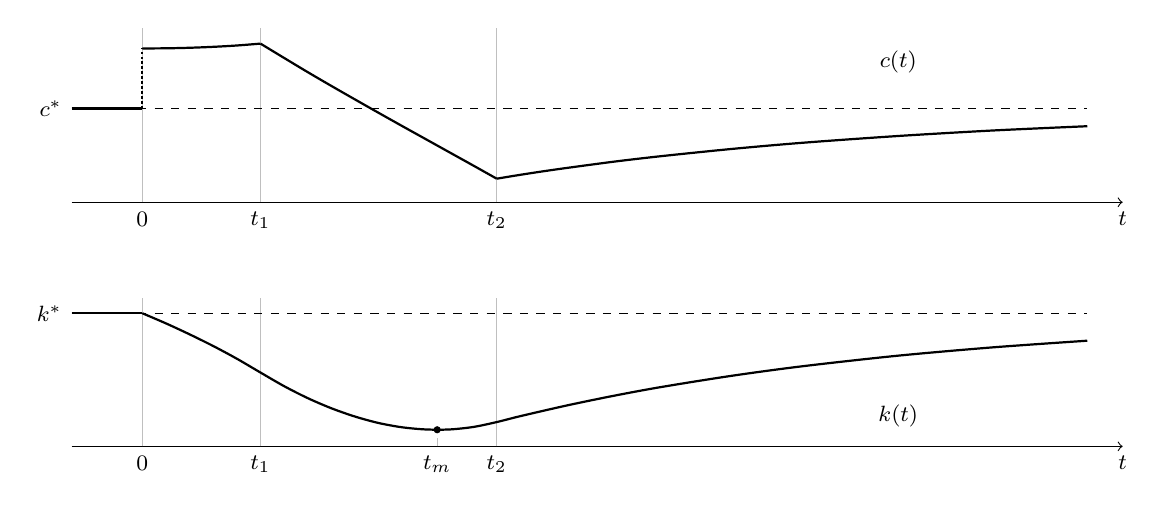
\begin{tikzpicture}[x=0.3cm,font=\footnotesize]
\begin{scope}[y=0.17cm]
  \draw[->] (-3,-7) -- (41.5,-7) node[below]{$t$};
  \foreach \x/\l in {0/0,5/t_1,15/t_2} \draw[gray!50] (\x,-7) node[below,black]{$\l$} -- (\x,6);
  \draw[dashed] (-3,0) node[left]{$c^*$} -- (40,0);
  \draw[thick] (-3,0) -- (0,0);
  \draw[thick,densely dotted] (0,0) -- (0,4.49);
  \draw[thick] plot[smooth] coordinates {(0,4.49) (1,4.50) (2,4.54) (3,4.61) (4,4.71) (5,4.85)};
  \draw[thick] plot[smooth] coordinates {(5,4.85) (6,3.78) (7,2.72) (8,1.69) (9,0.68) (10,-0.32) (11,-1.31) (12,-2.29) (13,-3.27) (14,-4.25) (15,-5.24)};
  \draw[thick] plot[smooth] coordinates {(15,-5.24) (16,-4.95) (17,-4.68) (18,-4.43) (20,-3.96) (22,-3.55) (25,-3.01) (28,-2.55) (32,-2.05) (36,-1.64) (40,-1.32)};
  \node at (32,3.5) {$c(t)$};
\end{scope}
\begin{scope}[yshift=-2.6cm,y=0.13cm]
  \draw[->] (-3,-13) -- (41.5,-13) node[below]{$t$};
  \foreach \x/\l in {0/0,5/t_1,15/t_2} \draw[gray!50] (\x,-13) node[below,black]{$\l$} -- (\x,1.5);
  \draw[gray!50,densely dashed] (12.48,-13) node[below,black]{$t_m$} -- (12.48,-11.38);
  \draw[dashed] (-3,0) node[left]{$k^*$} -- (40,0);
  \draw[thick] (-3,0) -- (0,0);
  \draw[thick] plot[smooth] coordinates {(0,0.00) (1,-0.99) (2,-2.06) (3,-3.20) (4,-4.44) (5,-5.79) (6,-7.12) (7,-8.29) (8,-9.28) (9,-10.09) (10,-10.72) (11,-11.14) (12,-11.35) (13,-11.35) (14,-11.11) (15,-10.63) (16,-10.05) (18,-8.99) (20,-8.04) (22,-7.19) (25,-6.09) (28,-5.16) (32,-4.14) (36,-3.33) (40,-2.68)};
  \fill (12.48,-11.38) circle (1.3pt);
  \node at (32,-10) {$k(t)$};
\end{scope}
\end{tikzpicture}\par
{\footnotesize (b): tax on $[5,15)$, announced at $0$. Same calibration and units as in (a).}
\end{center}

\intuicao{Anticipated policy moves the economy before it is implemented. Households know that saving will
be poorly rewarded during $[t_1,t_2)$, so consumption must fall over that window (Euler). Since $c$
cannot jump at $t_1$, the high level from which it falls must be built up beforehand, and under the
untaxed Euler equation consumption grows only if $f'(k)>\rho+\theta g$, i.e.\ only if capital is
already below $k^*$. So the economy starts to decumulate at the announcement, and consumption is
front-loaded relative to the tax period.}

\armadilha{(i) Letting $c$ jump when the tax starts or ends: both dates are known at $0$. (ii) In (a),
sending the economy to $S_T$: that answers the permanent tax of 2.10(b); with a temporary tax the target
is $S_N$ at $t_1$, and the economy is never on $S_T$. (iii) Claiming that $k$ falls during the whole
tax period: the landing point on $S_N$ lies below the $\dot k=0$ locus, so $k$ is already rising when
the tax ends. (iv) Shifting the $\dot k=0$ locus: it stays put because the revenue is rebated; it would
shift down if the revenue financed government purchases (2.10f).}

\refbib{Romer (2012), \S2.2--2.3 (eqs.~(2.17)--(2.18), (2.24)--(2.25), the saddle path), \S2.6 (an
unanticipated change: jump onto the new saddle path), \S2.7 (temporary versus permanent changes);
problems 2.10--2.11, pp.~95--96.}
\checado{\texttt{check-2-12-11-1.py} confirms symbolically that the rebate leaves $\dot k$ unchanged,
then simulates the calibrated economy by shooting $c_0$ for 2.10(b), 2.11 and both parts here, and
asserts every claim above: $c^*<c_0$, with jumps $100\ln(c_0/c^*)$ of $11.3$ (2.10b), $7.5$ (a) and
$4.5$ (b); the monotonicity of $c$ on each interval and the sign switch of $\dot c$ at the policy dates;
the minimum of $k$ at $t_m\approx8.4<t_1=10$ in (a) and at $t_m\approx12.5\in(5,15)$ in (b); and arrival
on $S_N$ (traced separately by backward integration) exactly at the last switch, with $c<c^*$, $k<k^*$.
Romer's solution manual (pp.~2-18--2-19) reaches the same answer for both parts.}
